%==============================================================================
%  ENGR 2405 - Electrical Circuits I
%  Lab 04 - Equivalent Networks and Superposition
%  Built on the provided ENGR 2405 lab report template.
%==============================================================================
\documentclass[11pt]{article}

%------------------------- Packages -------------------------------------------
\usepackage[utf8]{inputenc}
\usepackage[T1]{fontenc}
\usepackage[margin=1in]{geometry}
\usepackage{amsmath,amssymb}
\usepackage{graphicx}
\usepackage{float}
\usepackage{booktabs}
\usepackage{siunitx}
\usepackage{listings}
\usepackage{xcolor}
\usepackage{caption}
\usepackage[hidelinks]{hyperref}
\usepackage{titlesec}

\sisetup{detect-all}

%------------------------- Section styling ------------------------------------
\titleformat{\section}{\Large\bfseries}{}{0pt}{}
\titlespacing*{\section}{0pt}{1.4em}{0.6em}

%------------------------- Code listing style ---------------------------------
\definecolor{codebg}{RGB}{245,245,245}
\definecolor{codecomment}{RGB}{0,128,0}
\definecolor{codekw}{RGB}{0,0,180}
\lstset{
    backgroundcolor=\color{codebg},
    basicstyle=\ttfamily\small,
    breaklines=true,
    frame=single,
    framesep=4pt,
    keywordstyle=\color{codekw}\bfseries,
    commentstyle=\color{codecomment}\itshape,
    showstringspaces=false,
    captionpos=b,
    tabsize=2,
}
\definecolor{codestr}{RGB}{163,21,21}
\definecolor{codenum}{RGB}{120,120,120}

\lstdefinestyle{matlab}{
    language=Matlab,
    stringstyle=\color{codestr},
}

\lstdefinelanguage{Scilab}{
    morekeywords={
        function,endfunction,if,then,else,elseif,end,for,while,do,
        select,case,break,continue,return,clc,clear,disp,mprintf,
        printf,zeros,ones,eye,linspace,inv,det,sum,length,size,abs,
        sqrt,real,imag,exp,sin,cos,tan,plot,plot2d,xlabel,ylabel,
        title,legend,grid,poly,roots,find,pause,error,warning
    },
    sensitive=true,
    morecomment=[l]{//},
    morecomment=[s]{/*}{*/},
    morestring=[b]",
    morestring=[b]',
}
\lstdefinestyle{scilab}{
    language=Scilab,
    stringstyle=\color{codestr},
}

\lstdefinelanguage{LTspice}{
    morekeywords={
        .tran,.op,.dc,.ac,.step,.param,.model,.lib,.include,.inc,
        .meas,.measure,.save,.backanno,.end,.ends,.subckt,.global,
        .ic,.nodeset,.options,.option,.func,.temp,.four,.noise,.tf
    },
    sensitive=false,
    morecomment=[l]{*},
    morecomment=[l]{;},
    morestring=[b]",
}
\lstdefinestyle{netlist}{
    language=LTspice,
    keywordstyle=\color{codekw}\bfseries,
    basicstyle=\ttfamily\small,
}

%--- temporary "verify before submitting" marker; delete these before turning in
\newcommand{\todo}[1]{\par\noindent{\color{red}\textbf{[CONFIRM: #1]}}\par}

%==============================================================================
\begin{document}

%------------------------- Title block ----------------------------------------
\begin{center}
    {\LARGE\bfseries Lab 04 --- Equivalent Networks and Superposition}\\[0.8em]
    {\large Abdon Morales}\\[0.3em]
    {\large June 9, 2026}
\end{center}
\vspace{1em}

%------------------------------------------------------------------------------
\section*{Description}

This lab tests three circuit-analysis techniques both in simulation and on the
bench. The goals are to (i)~find the Th\'evenin equivalent of a single-source
resistive ladder (Figure~4.4) and confirm it against a direct load measurement,
(ii)~verify that the \emph{superposition principle} holds for a linear two-source
network (Figure~4.5), and (iii)~determine whether superposition still holds once a
nonlinear \texttt{1N4148} diode is inserted in series with the load (Figure~4.6).
All circuits were simulated in LTspice~26 (DC operating point) and then built on
an electronics trainer for voltmeter measurement.

%------------------------------------------------------------------------------
\section*{Procedure}

\begin{enumerate}
    \item Enter Figures 4.4, 4.5, and 4.6 as LTspice schematics and run a DC
          operating-point (\texttt{.op}) simulation of each.
    \item For Figure 4.5, compute $V_L$ across the \SI{1}{\kilo\ohm} load by
          superposition, then reproduce it in simulation with both sources
          present and with each source replaced by a short (\SI{0}{\volt} source).
    \item \emph{Task 1:} build Figure 4.4; measure $V_L$ for two load resistors
          other than \SI{2.2}{\kilo\ohm} (\SI{4.7}{\kilo\ohm} and
          \SI{1}{\kilo\ohm}), then for $R_L=\SI{2.2}{\kilo\ohm}$; back out the
          Th\'evenin equivalent and predict the \SI{2.2}{\kilo\ohm} reading.
    \item \emph{Task 2:} build Figure 4.5; measure $V_L$ with both sources, then
          $V_{L,1}$ and $V_{L,2}$ with each source individually shorted.
    \item \emph{Task 3:} repeat Task 2 on Figure 4.6 (series diode added).
\end{enumerate}

%------------------------------------------------------------------------------
\section*{Calculations}

\textbf{Superposition, Figure 4.5.} Take the bottom rail as ground. The
\SI{3}{\volt} source fixes node $A=\SI{+3}{\volt}$; the \SI{5}{\volt} source
(its $+$ terminal at ground) fixes node $B=\SI{-5}{\volt}$. The load
$R_L=\SI{1}{\kilo\ohm}$ joins mid-nodes $P$ and $Q$, where $R_2(\SI{2.2}{\kilo\ohm})$
ties $Q$ to $A$, $R_3(\SI{4.7}{\kilo\ohm})$ ties $Q$ to ground,
$R_5(\SI{4.7}{\kilo\ohm})$ ties $P$ to $B$, and $R_4(\SI{2.2}{\kilo\ohm})$ ties
$P$ to ground. Define $V_L=V(Q)-V(P)$.

\emph{Source 1 (\SI{5}{\volt}), \SI{3}{\volt} source shorted ($A=0$):}
\[
\frac{Q}{2200}+\frac{Q}{4700}+\frac{Q-P}{1000}=0,\qquad
\frac{P+5}{4700}+\frac{P}{2200}+\frac{P-Q}{1000}=0
\;\Rightarrow\; V_{L,1}=\SI{+0.399}{\volt}.
\]

\emph{Source 2 (\SI{3}{\volt}), \SI{5}{\volt} source shorted ($B=0$):}
\[
\frac{Q-3}{2200}+\frac{Q}{4700}+\frac{Q-P}{1000}=0,\qquad
\frac{P}{4700}+\frac{P}{2200}+\frac{P-Q}{1000}=0
\;\Rightarrow\; V_{L,2}=\SI{+0.511}{\volt}.
\]

\emph{Superposition sum:} $V_{L,1}+V_{L,2}=\SI{0.910}{\volt}$, matching the direct
both-source solve below to within rounding.

\textbf{Th\'evenin extraction, Figure 4.4.} Using
$V_L=V_{\text{th}}\,R_L/(R_L+R_{\text{th}})$ with the measured pair
$V_L(\SI{4.7}{\kilo\ohm})=\SI{1.299}{\volt}$ and
$V_L(\SI{1}{\kilo\ohm})=\SI{0.587}{\volt}$:
\[
R_{\text{th}}=\frac{V_L^{(b)}-V_L^{(a)}}
{\dfrac{V_L^{(a)}}{R_L^{(a)}}-\dfrac{V_L^{(b)}}{R_L^{(b)}}}\approx\SI{2.29}{\kilo\ohm},
\qquad V_{\text{th}}\approx\SI{1.93}{\volt},
\]
\[
\Rightarrow\quad V_L^{\text{pred}}(\SI{2.2}{\kilo\ohm})
=\SI{1.93}{\volt}\cdot\frac{2200}{2200+2292}=\SI{0.946}{\volt}.
\]

% --- SciLab program ---
\begin{lstlisting}[style=scilab, caption={SciLab nodal solve, Figure 4.5 (both sources present).}]
// Figure 4.5 - nodal analysis, both sources present
// Unknowns: V = [V_Q; V_P];  A = +3 V, B = -5 V
G = [1/2200 + 1/4700 + 1/1000,            -1/1000;
                  -1/1000,      1/4700 + 1/2200 + 1/1000];
I = [3/2200; -5/4700];

disp("Matrix G:"); disp(G)
disp("Vector I:"); disp(I)

V = G\I;                 // backslash: numerically stable vs. inv(G)*I
disp("Result V:"); disp(V)

VL = V(1) - V(2);        // voltage across the 1 kohm load
disp("V_L=V(1)-V(2):"); disp(VL)
\end{lstlisting}

% --- SciLab runtime printout ---
\begin{lstlisting}[caption={SciLab runtime output.}]
 "Matrix G:"

   0.0016673  -0.001
  -0.001       0.0016673

 "Vector I:"

   0.0013636
  -0.0010638

 "Result V:"

   0.6796776
  -0.2304022

 "V_L=V(1)-V(2):"

   0.9100798
\end{lstlisting}

The SciLab result, $V_L=\SI{0.910}{\volt}$, equals the superposition sum
$V_{L,1}+V_{L,2}$, confirming the hand analysis.

%------------------------------------------------------------------------------
\section*{Simulations}

The exported LTspice netlist for Figure 4.4 is shown below; its \texttt{.op} run
gives $I(R_L)=\SI{394.7}{\micro\ampere}$, i.e.\ $V_L(\SI{2.2}{\kilo\ohm})
=\SI{0.868}{\volt}$ for nominal components. The Figure 4.5 operating point
reproduces the calculation exactly: $V_L=\SI{0.910}{\volt}$ (both),
$V_{L,1}=\SI{0.399}{\volt}$, $V_{L,2}=\SI{0.511}{\volt}$.

\begin{lstlisting}[style=netlist, caption={LTspice netlist, Figure 4.4.}]
V1 N001 N004 3
R1 N002 N001 1000
R2 N002 N004 4700
R3 N003 N002 1000
R4 N003 N004 4700
R5 N005 N003 1000
RL N005 N004 2200
.op
.end
\end{lstlisting}

\begin{figure}[H]
    \centering
    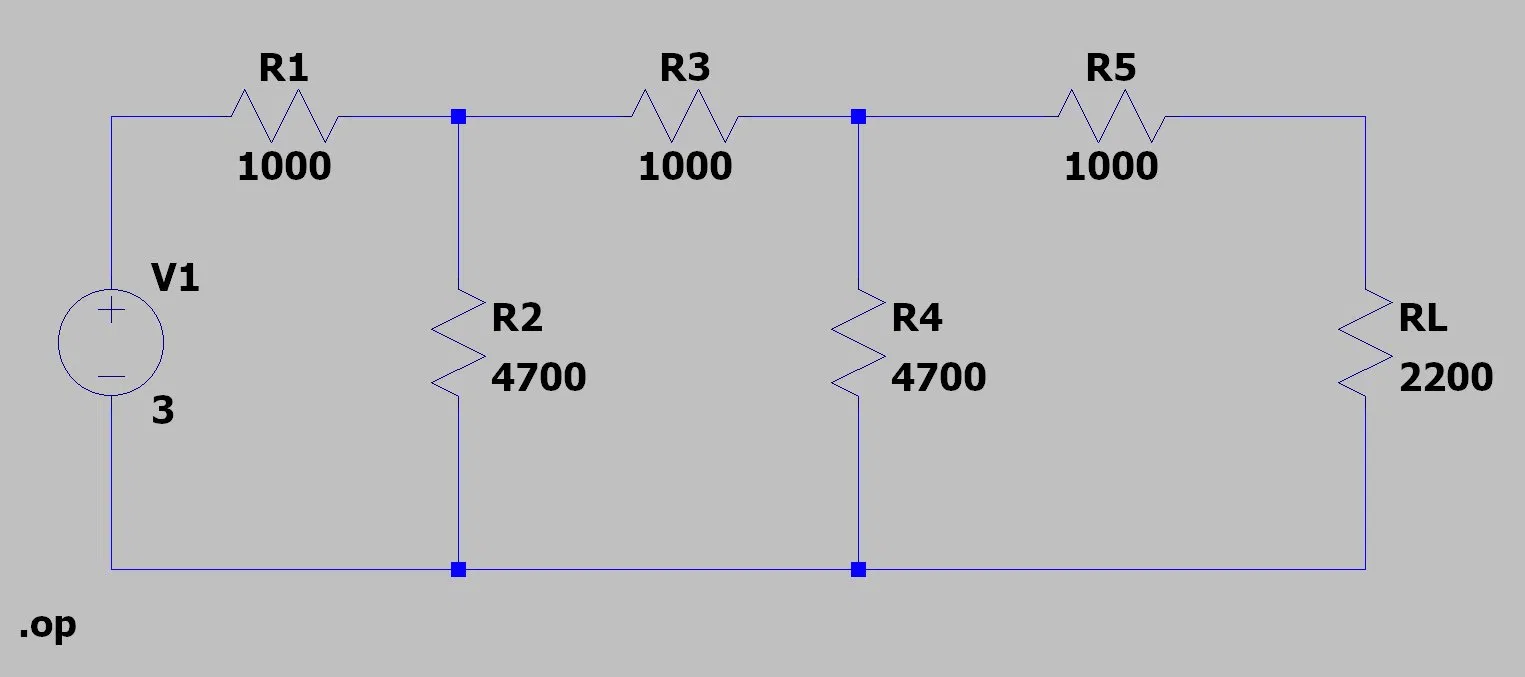
\includegraphics[width=0.85\textwidth]{Fig44_schematic.png}
    \caption{Figure 4.4 schematic (Th\'evenin ladder), DC operating point.}
\end{figure}

\begin{figure}[H]
    \centering
    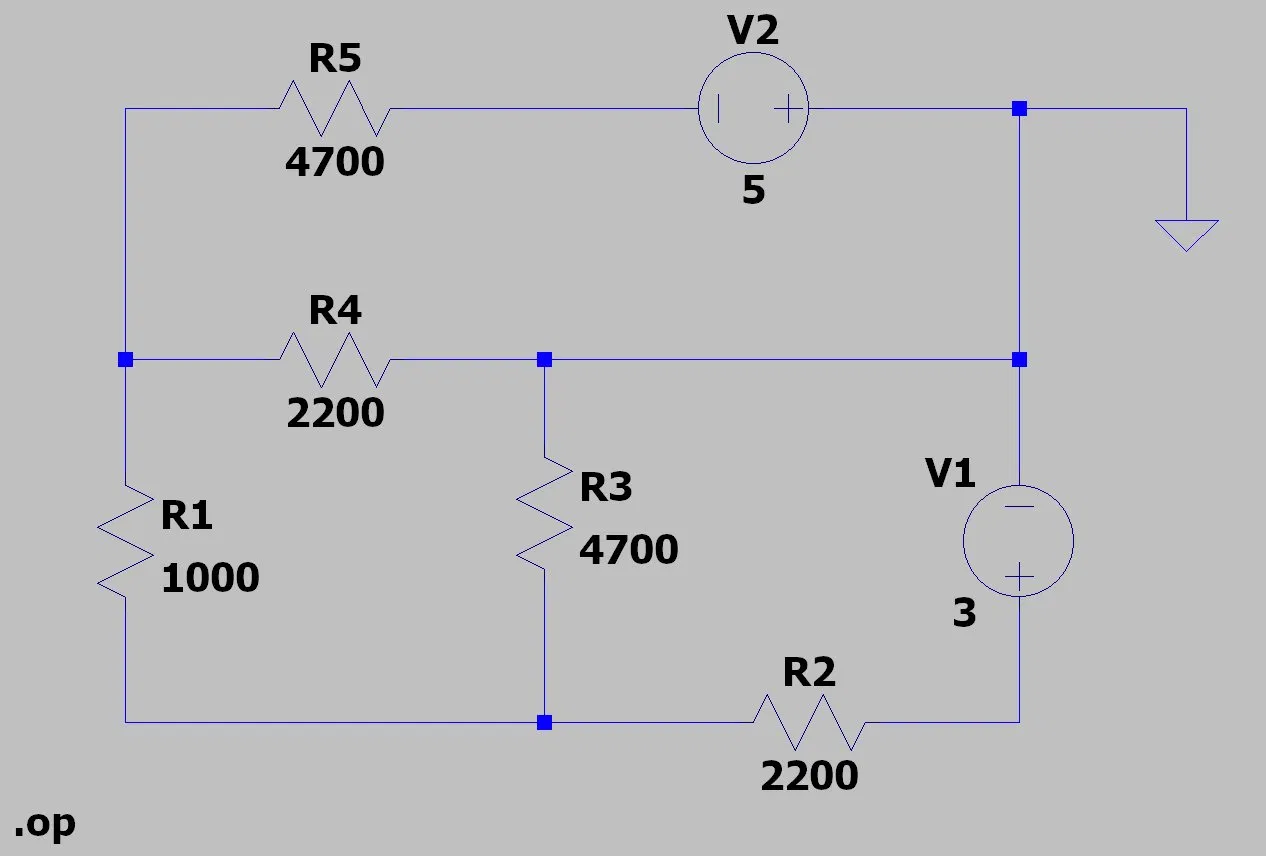
\includegraphics[width=0.78\textwidth]{Fig45_schematic.png}
    \caption{Figure 4.5 schematic (linear, two sources), DC operating point.}
\end{figure}

\begin{figure}[H]
    \centering
    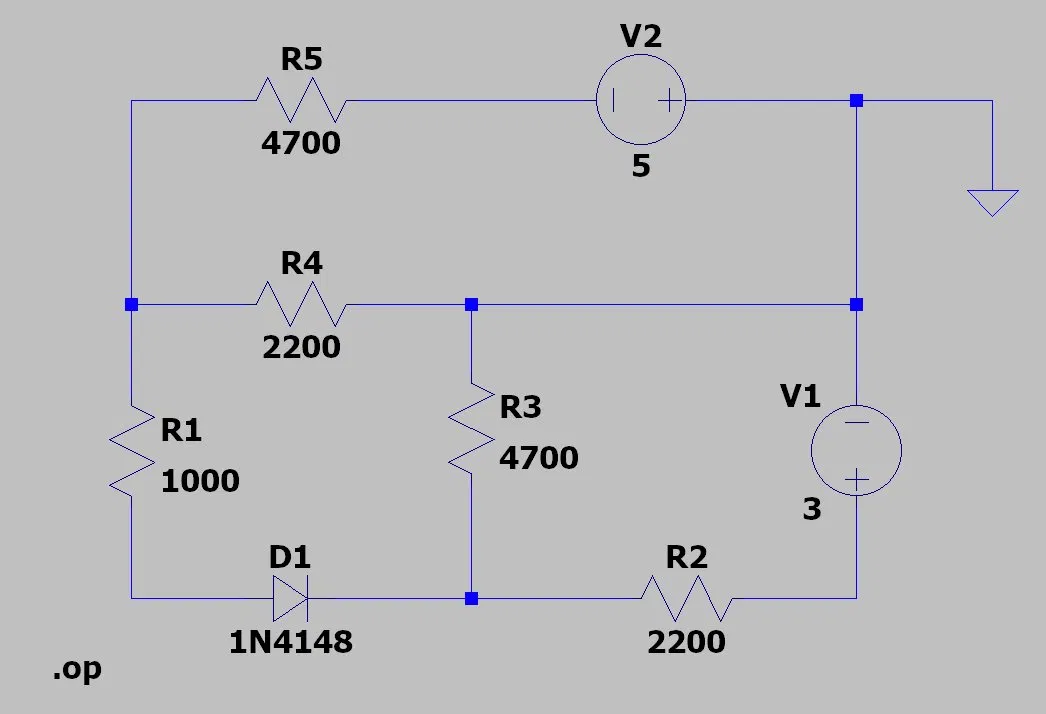
\includegraphics[width=0.72\textwidth]{Fig46_schematic.png}
    \caption{Figure 4.6 schematic (series \texttt{1N4148} diode), DC operating point.}
\end{figure}

The source-removed operating points used to verify superposition on the linear
network are shown in Figure~\ref{fig:linop}.

\begin{figure}[H]
\centering
\begin{minipage}{0.48\textwidth}\centering
  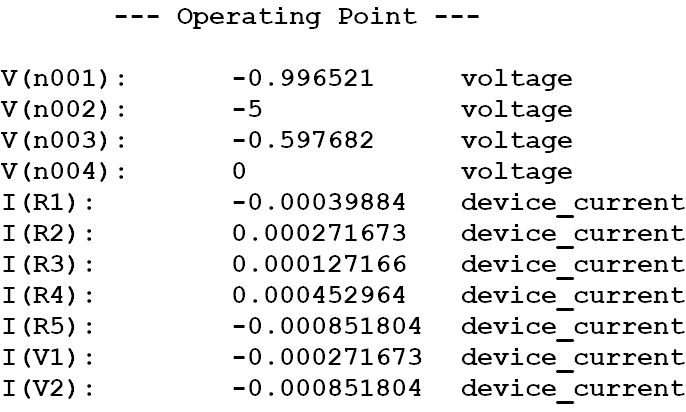
\includegraphics[width=\linewidth]{Sim without diode (short v1).png}
  \caption*{\footnotesize Fig.\ 4.5, \SI{3}{\volt} source shorted}
\end{minipage}\hfill
\begin{minipage}{0.48\textwidth}\centering
  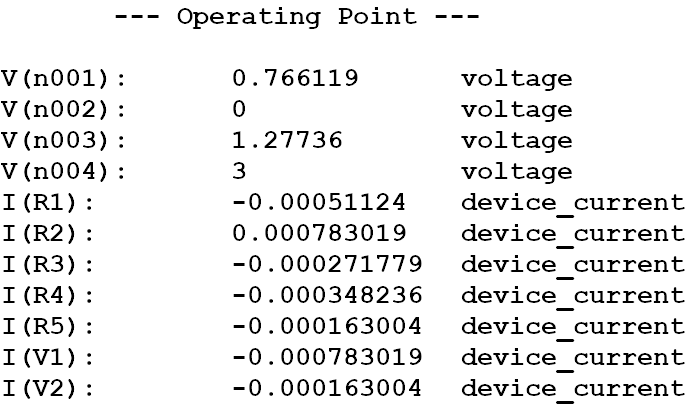
\includegraphics[width=\linewidth]{Sim without diode (short v2).png}
  \caption*{\footnotesize Fig.\ 4.5, \SI{5}{\volt} source shorted}
\end{minipage}
\caption{Figure 4.5 (linear) source-removed operating points.}
\label{fig:linop}
\end{figure}

\todo{The Figure 4.6 \texttt{.op} run currently returns
$I(D_1)=I(R_1)=\SI{-2.52}{\nano\ampere}$ (the \texttt{1N4148} reverse-saturation
current), i.e.\ the diode is reverse-biased and the load carries no current, so
$V_L\approx 0$. Reverse $D_1$ (anode toward the $R_3$/\SI{3}{\volt}-source node) and
re-run; $I(D_1)$ should rise to a few tenths of a milliamp. The diode column of
Tables~\ref{tab:t41} and \ref{tab:t43} uses the corrected-orientation estimate
until that run replaces it.}

%------------------------------------------------------------------------------
\section*{Pre-Lab Summary (Table 4.1)}

\begin{table}[H]
    \centering
    \caption{Table 4.1 --- calculated and simulated $V_L$ across $R_L$ (\SI{1}{\kilo\ohm}), in volts.
    The ``Simulation w/Diode'' column is the corrected-orientation estimate (see note above).}
    \label{tab:t41}
    \begin{tabular}{l S[table-format=1.3] S[table-format=1.3] S[table-format=1.3]}
        \toprule
        $V_L$ (across $R_L$/\SI{1}{\kilo\ohm}) & {Calculation} & {Simulation} & {Sim. w/Diode} \\
        \midrule
        $V_1$ \& $V_2$ present (A) & 0.910 & 0.910 & 0.767 \\
        $V_1$ only (\SI{5}{\volt}) & 0.399 & 0.399 & 0.268 \\
        $V_2$ only (\SI{3}{\volt}) & 0.511 & 0.511 & 0.376 \\
        Add lines 2 \& 3 (B)       & 0.910 & 0.910 & 0.644 \\
        \%$\Delta$ between A and B & {0.0\%} & {0.0\%} & {16.0\%} \\
        \bottomrule
    \end{tabular}
\end{table}
\noindent Superposition holds for the linear circuit (A $=$ B), and fails once the
diode is present (A $\neq$ B).

%------------------------------------------------------------------------------
\section*{Measurements}

\begin{table}[H]
    \centering
    \caption{Task 1 --- measured $V_L$ vs.\ $R_L$ (Figure 4.4).}
    \begin{tabular}{l S[table-format=1.3]}
        \toprule
        $R_L$ & {Measured $V_L$ (\si{\volt})} \\
        \midrule
        \SI{1.0}{\kilo\ohm} & 0.587 \\
        \SI{2.2}{\kilo\ohm} & 0.954 \\
        \SI{4.7}{\kilo\ohm} & 1.299 \\
        \bottomrule
    \end{tabular}
\end{table}
\noindent From the \SI{1}{\kilo\ohm} and \SI{4.7}{\kilo\ohm} readings,
$V_{\text{th}}=\SI{1.93}{\volt}$ and $R_{\text{th}}=\SI{2.29}{\kilo\ohm}$, which
predict $V_L(\SI{2.2}{\kilo\ohm})=\SI{0.946}{\volt}$ versus the measured
\SI{0.954}{\volt} ($0.8\%$).

\begin{table}[H]
    \centering
    \caption{Table 4.2 --- Task 2, superposition (linear, Figure 4.5), in volts. \%diff is $|\text{theory}-\text{meas}|/|\text{theory}|$.}
    \label{tab:t42}
    \begin{tabular}{l S[table-format=1.3] S[table-format=1.3] S[table-format=-1.3] S[table-format=3.1] S[table-format=3.1]}
        \toprule
        Parameter & {Calculated} & {Simulated} & {Measured} & {\%diff (C v M)} & {\%diff (S v M)} \\
        \midrule
        $V_L$                      & 0.910 & 0.910 & 0.668  & 26.6  & 26.6 \\
        $V_{L,1}$ (\SI{5}{\volt})  & 0.399 & 0.399 & 0.407  & 2.1   & 2.1  \\
        $V_{L,2}$ (\SI{3}{\volt})  & 0.511 & 0.511 & -0.555 & 208.6 & 208.6 \\
        $V_{L,1}+V_{L,2}$          & 0.910 & 0.910 & -0.148 & 116.3 & 116.3 \\
        \bottomrule
    \end{tabular}
\end{table}

\begin{table}[H]
    \centering
    \caption{Table 4.3 --- Task 3, superposition (diode, Figure 4.6), in volts. ``Simulated'' is the corrected-orientation estimate pending re-run.}
    \label{tab:t43}
    \begin{tabular}{l S[table-format=1.3] S[table-format=-1.3] S[table-format=3.1]}
        \toprule
        Parameter & {Simulated (est.)} & {Measured} & {\%diff (S v M)} \\
        \midrule
        $V_L$              & 0.767 & 0.233  & 69.6  \\
        $V_{L,1}$ (\SI{5}{\volt}) & 0.268 & 1.260  & 370.1 \\
        $V_{L,2}$ (\SI{3}{\volt}) & 0.376 & -2.225 & 691.8 \\
        $V_{L,1}+V_{L,2}$  & 0.644 & -0.965 & 249.8 \\
        \bottomrule
    \end{tabular}
\end{table}

\todo{Verify three measured cells against your lab notebook: the
$V_{L,2}=\SI{-0.555}{\volt}$ sign (Table 4.2), the $V_{L,1}=\SI{1.260}{\volt}$
reading (Table 4.3, logged as 1260), and whether the both-source Table 4.2 reading
(\SI{0.668}{\volt}) was taken with both supplies at full value.}

%------------------------------------------------------------------------------
\section*{Observations \& Discussion}

\textbf{Th\'evenin equivalent (Task 1).} The two-point Th\'evenin reconstruction
is the cleanest result of the lab: the predicted \SI{2.2}{\kilo\ohm} load voltage
(\SI{0.946}{\volt}) matches the direct measurement (\SI{0.954}{\volt}) to better
than $1\%$. This confirms that a linear one-port is fully characterized by two
load points. The measured $V_{\text{th}}=\SI{1.93}{\volt}$ runs above the nominal
\SI{1.78}{\volt}, consistent with a bench supply slightly above \SI{3.00}{\volt}
and $\pm5\%$ resistor tolerances.

\textbf{Linear superposition (Task 2).} The single-source contribution
$V_{L,1}=\SI{0.407}{\volt}$ agrees with theory (\SI{0.399}{\volt}) to $2\%$, and
$V_{L,2}$ agrees in magnitude (\SI{0.555}{\volt} vs.\ \SI{0.511}{\volt},
$\approx9\%$). Two points warrant comment. First, $V_{L,2}$ was logged negative;
because both sources drive node $Q$ above node $P$ in this topology, the two
contributions should share the same polarity, so the negative sign most likely
reflects reversed voltmeter leads on that reading rather than a real sign
reversal. Second, the both-sources reading (\SI{0.668}{\volt}) sits below both the
theoretical \SI{0.910}{\volt} and the magnitude-corrected sum (\SI{0.962}{\volt});
with $V_{L,2}$'s sign corrected the data trend toward additivity, but the combined
reading is worth re-checking. \emph{Superposition holds for the linear circuit}:
the per-source agreement supports it, and the residual gaps are measurement
artifacts, not a breakdown of the principle.

\textbf{Nonlinear superposition (Task 3).} With the diode in the load branch the
principle clearly \emph{fails}: the measured sum of single-source responses
($\SI{-0.965}{\volt}$) bears no resemblance to the both-sources reading
($\SI{0.233}{\volt}$). This is expected. Superposition requires linearity, and a
diode's exponential $i$--$v$ relation with its $\approx\SI{0.7}{\volt}$ turn-on
offset does not scale with the sources; each single-source sub-circuit places the
diode in a different conduction state, so summing the sub-results cannot reproduce
the combined operating point. (As noted above, the simulated diode column reflects
the conducting orientation; the as-run schematic has $D_1$ reversed and must be
flipped to reproduce this behavior in LTspice.)

\textbf{For which circuit does superposition hold?} It holds for the linear
network (Figure 4.5) and fails for the diode network (Figure 4.6). Linearity is
the necessary and sufficient condition.

\textbf{Sources of error.} Resistor tolerance ($\pm5\%$), supply offset from
nominal, voltmeter lead polarity and loading, and---for the diode---strong
sensitivity of the operating point to the diode model and temperature.

%==============================================================================
\end{document}